\chapter{Исследовательская часть}

В данном разделе будут приведены примеры работы программы, а также проведен сравнительный анализ процессорного времени работы реализаций алгоритмов при различных ситуациях на основе полученных данных.

\section{Технические характеристики}

Технические характеристики устройства, на котором выполнялись замеры времени, представлены далее:

\begin{itemize}
	\item операционная система Windows 11 Pro Версия 22H2 (22621.674) \cite{wind};
	\item память 16 ГБ;
	\item процессор 11th Gen Intel(R) Core(TM) i5-11400 2.59 ГГц \cite{proc}, 6 физических и 12 логических ядер.
\end{itemize}

При тестировании компьютер был включен в сеть электропитания. Во время замеров процессорного времени устройство было нагружено только встроенными приложениями окружения, а также системой тестирования.

\section{Демонстрация работы программы}

На рисунке \ref{img:res} представлен результат работы программы. Работающая программа выводит на экран журнал отладки для каждой заявки.
%\newpage
\begin{center}
	\centering{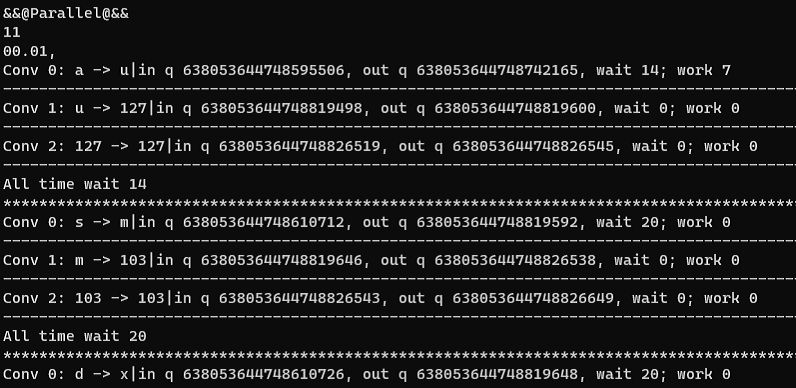
\includegraphics[trim=0 0 0cm 0cm bb=0 0 1008 786, scale=0.75]{src/screen}}
	\captionof{figure}{Пример работы программы}
	\label{img:res}
\end{center}

\section{Время выполнения реализаций алгоритмов}

\textbf{Входные данные:} 10000 строк, размером от 500 до 2500 символов.

В таблице ниже приведены результаты замеров времени (в тиках) для общего времени пребывания заявок в очередях.

\begin{center}
	\begin{threeparttable}
		\caption{Суммарное время пребывания всех заявок в очереди в тиках $* 10^{-5}$}
		\label{tbl:best}
		\begin{tabular}{|c|c|c|}
			\hline
			Длина входных строк &Линейный конвейер &Параллельный конвейер\\
			\hline
			500 & 33102498& 15664766 \\
			\hline
		    1000& 105645693 &49704767 \\
		    \hline
		    2000&364612686 & 185795895\\
			\hline
		    2500 & 536216748&276675101 \\
			\hline
		\end{tabular}
		
	\end{threeparttable}
\end{center}


 На рисунке \ref{img:graph_sorted} приведены графические результаты замеров времени работы алгоритмов в зависимости от линейного размера входной строки.

\begin{center}
	\centering{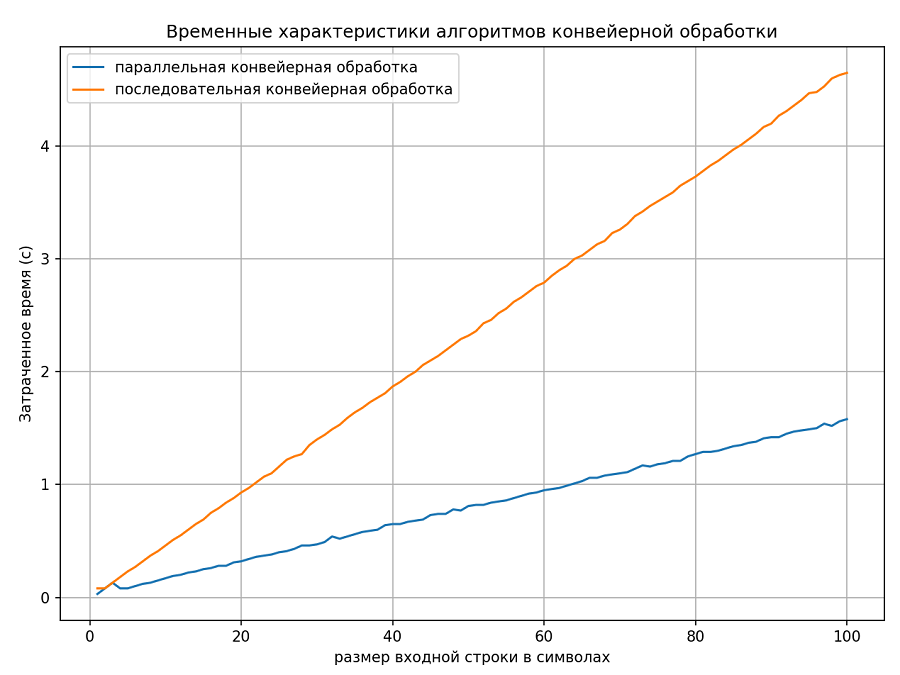
\includegraphics[trim=0 0 0 -5cm bb=0 0 800 800, scale=0.75]{src/good}}
	\captionof{figure}{Время вычислений}
	\label{img:graph_sorted}
\end{center}





\section{Вывод}
По полученным результатам иследования можно сделать вывод, что конвейер выигрывает от двух до трех раз в скорости работы и снижении времени ожидания заявок в очереди перед линейной реализацией.
